\documentclass{article}
\usepackage{fancyhdr} 
\usepackage{lastpage}
\usepackage{mathtools}
\usepackage{extramarks}
\usepackage{graphicx}
\usepackage{listings}
\usepackage{courier}
\usepackage{lipsum} 
\usepackage{enumerate}
\usepackage{amsmath}
\usepackage{url}
\usepackage{caption}

% Margins
\topmargin=-0.45in
\evensidemargin=0in
\oddsidemargin=0in
\textwidth=6.5in
\textheight=9.0in
\headsep=0.25in
\linespread{1.1} % Line spacing

% Set up the header and footer
\pagestyle{fancy}
\lhead{COMP3308}
\chead{Introduction to Artificial Intelligence}
\rhead{Assignment 2}
\lfoot{}
\cfoot{\thepage}
\rfoot{Woo Hyun Jung 310250811 \\  Khanh Cao Quoc Nguyen 311253865} 
\renewcommand\headrulewidth{0.4pt}
\renewcommand\footrulewidth{0.4pt}
\renewcommand{\tt}{\texttt}
\setlength\parindent{0pt} 

\title{COMP3308 Assignment 2 \\ Bayesian Networks}
\author{Woo Hyun Jung 310250811 \\  Khanh Cao Quoc Nguyen 311253865}
\date{}
\begin{document}
\maketitle
\thispagestyle{empty}
\newpage

\section{Aim}
blah blah blah blah blah blah blah blah blah blah blah blah blah blah blah blah blah blah blah blah blah blah blah blah blah blah blah blah blah blah blah blah blah blah blah blah blah blah blah blah blah blah blah blah blah blah blah blah blah blah blah blah blah blah blah blah blah blah blah blah blah blah blah blah blah blah blah blah blah blah blah blah blah blah blah blah blah blah blah blah blah blah blah blah blah blah blah blah blah blah blah blah blah 

\section{Methods}
\subsection{Bayesian Networks}
Bayesian networks are simple, probabilistic graphical models that represent sets of random variables and their conditional dependencies.

\subsection{Variable Elimination}
blah blah blah blah blah blah blah blah blah blah blah blah blah blah blah blah blah blah blah blah blah blah blah blah blah blah blah blah blah blah blah blah blah blah blah blah blah blah blah blah blah blah blah blah blah blah blah blah blah blah blah blah blah blah blah blah blah blah blah blah blah blah blah blah blah blah blah blah blah blah blah blah blah blah blah blah blah blah blah blah blah blah blah blah blah blah blah blah blah blah blah blah blah 

\subsection{Likelihood Weighting}
blah blah blah blah blah blah blah blah blah blah blah blah blah blah blah blah blah blah blah blah blah blah blah blah blah blah blah blah blah blah blah blah blah blah blah blah blah blah blah blah blah blah blah blah blah blah blah blah blah blah blah blah blah blah blah blah blah blah blah blah blah blah blah blah blah blah blah blah blah blah blah blah blah blah blah blah blah blah blah blah blah blah blah blah blah blah blah blah blah blah blah blah blah 

\section{Results and Discussion}
\subsection{Question 1}

Metastatic cancer is a possible cause of a brain tumour and is also an explanation for increased total serum calcium. In turn, either of these could explain a patient falling into a coma. Severe headache is also possibly associated with a brain tumour. 

\begin{itemize}
\item The prior probability of metastatic cancer $P(m)$ is 0.2. 
\item The conditional probability of increased total serum calcium $P(I | M)$ is: $P(i | m) = 0.8$ and $P(i | \neg m) = 0.2$ 
\item The conditional probability of brain tumor $P(B | M)$ is: $P(b | m) = 0.2$ and $P(b | \neg m) = 0.05$ 
\item The conditional probability of coma $P(C | I, B)$ is: $P(c | i, b) = 0.8$, $P(c | \neg i, b) = 0.8$, $P(c | i, \neg b) = 0.8$ and $P(c | \neg i, \neg b) = 0.05$. 
\item The conditional probability of severe headache $P(S | B)$ is $P(s | b) = 0.8$ and $P(s | �b) = 0.6$.
\end{itemize} 

\begin{enumerate}[a)]
\item Construct and show the equivalent graphical model.
\begin{figure}
\begin{center}
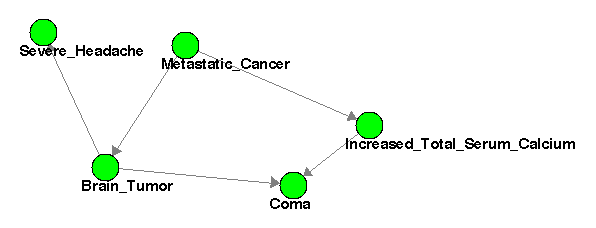
\includegraphics[scale=0.7]{part1_bn}
\caption{Equivalent graphical model created using JavaBayes}
\end{center}
\end{figure}

\item What is the prior probability of coma $P(C)$?

\begin{minipage}{\linewidth}
\begin{lstlisting}
Posterior distribution:
	probability (  "Coma" ) { //1 variable(s) and 2 values
		table 
			0.47435035514892876	// p(true | evidence )
			0.5256496448510712; 	// p(false | evidence );
	}
\end{lstlisting}
\captionof{figure}{Probability of coma query output using JavaBayes}
\end{minipage}\\
\\
\\
Using the \tt{Query} function in JavaBayes, $P(C) = 0.47435035514892876$.

\item What is the probability of metastatic cancer given the patient has severe headaches and has not fallen into coma? 

\begin{minipage}{\linewidth}
\begin{lstlisting}
Posterior distribution:
	probability (  "Metastatic_Cancer" ) { //1 variable(s) and 2 values
		table 
			0.0757614259265982	// p(true | evidence )
			0.9242385740734018; 	// p(false | evidence );
	}
\end{lstlisting}
\captionof{figure}{$P(M | S, \neg C)$ query output using JavaBayes}
\end{minipage}\\
\\
\\
Using the \tt{Query} function in JavaBayes, $P(M | S, \neg C) = 0.0757614259265982$.

\item What is the Markov blanket of coma?

In a Bayesian network, the Markov blanket of node A includes its parents, children and the other parents of all of its children.

Therefore the Markov blanket of coma are brain tumor and increased total serum calcium.

\item Are increased total serum calcium and brain tumor independent given coma? Explain.

No, because of explaining away otherwise known as Berkson's Paradox.

Normally, total serum calcium and brain tumor are independent, but if we are given coma they become dependent since they share the same child.

\item What is the probability of fallen into coma given the patient has metastatic cancer? 

\begin{minipage}{\linewidth}
\begin{lstlisting}
Posterior distribution:
	probability (  "Coma" ) { //1 variable(s) and 2 values
		table 
			0.5040679804736937	// p(true | evidence )
			0.4959320195263062; 	// p(false | evidence );
	}
\end{lstlisting}
\captionof{figure}{$P(C | M)$ query output using JavaBayes}
\end{minipage}\\
\\
\\
Using the \tt{Query} function in JavaBayes, $P(C | M) = 0.5040679804736937$.
\end{enumerate} 

\subsection{Question 2}

\subsection{Question 3}

\subsection{Question 4}










\section{Conclusions}

\section{Reflection}

\section{Instructions}













\end{document}